\chapter{Adversarial attacks, imbalanced learning and domain shift}

This chapter focuses on how adversarial attacks are set out to successfully exploit the CNNs caveats explained in the last chapter. It starts with a study on the origin of adversaries and how imbalanced data and domain shift affect general predictive models accuracy. The discussion follows on different types of \textit{gradient sign} methods and how they use internal model information to create intentional perturbation on images. We finally end the chapter by presenting two different categories of perturbation and their interpretation on adversarial attacks.
\section{Why adversaries exist?}

Understanding why adversarial samples exists requires exploration of how learning models are built. The training data is a corpus of samples taken from an expected input distribution that are labeled according to their true class. For instance, one could have a set of e-mails classified as spam and not spam or a collection of pictures of animals where the label corresponds to each true animal type.

The integrity of CNNs is usually measured by how accurate the model is when performing a classification task. This metric is of paramount importance and, therefore, is a common target for techniques trying to exploit model vulnerabilities. Specifically, an adversary of a CNN seeks to provide an input X' that results in incorrect output classification. The degree of incorrectness in the prediction can vary and, therefore, impacts the classifier output in different ways.

Adversary types could be classified by four different categories as discussed by \cite{papernot_thesis_2016}. Confidence reduction is the adversary potential to introduce class ambiguity by reducing classification confidence. For instance, an input predicted with 99\% of confidence could have this level reduced without affecting the actual output of the model. Misclassification, on the other hand, happens when a label being previously correct is randomly changed to an incorrect output label, affecting the model output. Another different type of misclassification is to actually create perturbations using a specific target class, this method forces the model to predict towards that class. Finally, one could use the same class to create perturbations that makes the class looks less likely itself, moving the prediction outcome to the nearest class in the data space.

\section{Learning from imbalanced data}

In general, neural networks algorithms are designed to assume that the number of samples in a specific class label are roughly similar. Nevertheless, this scenario is often rare on the real world, as in most cases, the data distribution available is skewed and, hence, causes the model to be biased towards the labels with higher number of data points. This problem is known as learning from imbalanced data \cite{japkowicz2002class} and points to critical questions that are yet to be answered so one can gain deeper understanding of the vast field of machine learning. Generally speaking, there are three main approaches to learning from imbalanced data \cite{krawczyk2016learning}. 
\begin{itemize}
	\item Data-level: Aims to manipulate the data distribution by performing oversampling and undersampling operations to make it suitable for a standard learning algorithm
	\item Algorithm-level: Concentrates on modifying existing techniques to prevent bias towards majority classes and incorporate, for instance, varying penalties for each individual group of examples.
	\item Hybrid: Combines the advantages of the two previous approaches.
\end{itemize}

Even though there has been continuous development on learning from imbalanced data, there are still some new emerging challenges in, more specifically, highly dimensional data domains. As the number of dimensions of the training dataset grows, the difficulty into occupying the data space properly also increases. Varied forms of learning such as supervised, unsupervised and regression suffer from data imbalance. Moreover, extensive research on real-life applications shows that uneven data representation is an ongoing problem \cite{krawczyk2016learning}.

\section{Domain shift}



Classification accuracy should be carefully measured when training a model. For instance, the accuracy value obtained from the training set is usually higher than the one obtained from the test set. This happens when the joint distributions of training and test stages are different. A poor performance on the test set means that the divergence of both distributions (training and test domains) is high. This phenomena is usually known as domain shift or dataset shift \cite{Quionero}

Regardless of the technique, a machine learning model represents an approximation of the phenomena being modeled. In most cases the training data is unable to represent all possible input feature vectors and, therefore, can not fully capture a complete understanding of the target domain. A problem arises when the system can be exploited by providing samples that are not within the aforementioned input domain. They usually use information about the system to find where the model is inaccurate owing to missing items of the given training set.

What adversaries do is to force the domain shift in a way that the model is unable to generalize well on test data. Since data in most circumstances can not cover the entire feature space, the real decision boundary of a classification model generally becomes more complex as the phenomenon becomes more nuanced and the feature and dimension space becomes larger. This complexity is exploited by adversaries through the use of the model error as a guideline for perturbing a sample.

\begin{figure}[!h]
	\centering
	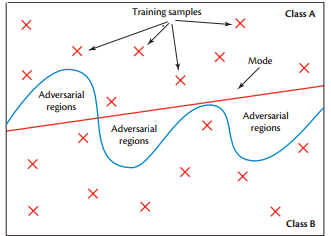
\includegraphics[scale=1.0]{adv_space.png}
	\caption{Two Dimensional Representation of unexplored adversarial regions \cite{papernot_2017}}
	\label{fig:adv_space}
\end{figure}

\section{Fast gradient sign method - FGSM}

The fast gradient sign method developed by \cite{goodfellow2014} has been used as the foundation of many of the experiments in adversarial learning on CNNs. The results have led to the conclusion that CNNs have linear behavior in very high dimensional spaces.  Most inputs were miss-classified not only on \cite{goodfellow2014} experiments but many others as well \cite{billovits, papernot2016, goodfellow2016}. This shows that adversarial examples are not hard to find. The method uses gradient information to generate image noises that changes classification outputs.
\begin{equation}
C(x + \delta)\approx C(x) + \delta * sign(\nabla C)
\end{equation}

The gradient sign equation has a simple interpretation. The main goal is to add a change $\delta$ into each pixel of the image so as to make that image closer to the chosen label on which we extracted the gradient from the source network. The sign on our $\nabla C$ indicates that we are only interested on the direction of the gradient while the $\epsilon$ controls the magnitude of the step. The method adds intentional noise that emphasizes the pixels in the image with the highest importance, so the resulting perturbation can likely lead to a misclassified result. By using the \textit(sign) function of the gradient, it is assured that the value will grow linearly with the number of the dimensions \cite{goodfellow2014}. The result of many small pixel changes is likely to generate an image with a wrong label in the network output.

The method exploits the loss function in an optimization process so one can maximize any class score for a given input image. Since everything in a CNN is differentiable it is relatively straight forward to compute the gradient information of any specific class of the input domain. The process can be done by doing a forward pass on a network with the desired class output being set to 1 in the final layer, then the backpropagation retrieves the necessary changes on gradients that would make any image looks like the desired class. 

Billovits et al (2016) summarized four different categories of adversarials generated by FGSM. True Adversarial are those given a completely different label after being perturbed. Re-Focused adversarial is the method that changes the focus of an image by giving a classification of an object that used to have lower significance while keeping the original object presence. Conaturally adversarial are those where the new output has some close relation to the miss-classified result (e.g. Dog and Cat). Finally, benign adversarial happens when the model misses the top prediction of the original image but the adversarial example gets randomly classified correctly with high confidence.

\begin{figure}[!h]
	\centering
	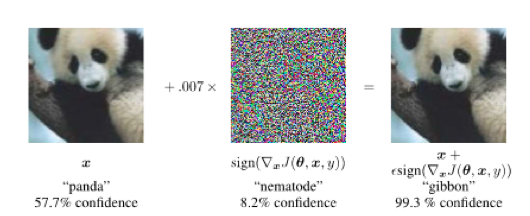
\includegraphics[scale=0.6]{panda.png}
	\caption{Adversarial example crafting with fast gradient sign \cite{goodfellow2014}.}
	\label{fig:fgsm_craft}
\end{figure}

\section{Iterative gradient sign method - IGSM}

The method from the previous section shows that small perturbations can intentionally change classifiers class labels. Sometimes, more than one iteration of the gradient sign method is required in order to have an image being incorrectly classified. By progressively applying small perturbations to an image one could achieve miss-classification of the desired sample that was not affected by one single iteration \cite{goodfellow2016}. 

\begin{figure}[!h]
	\centering
	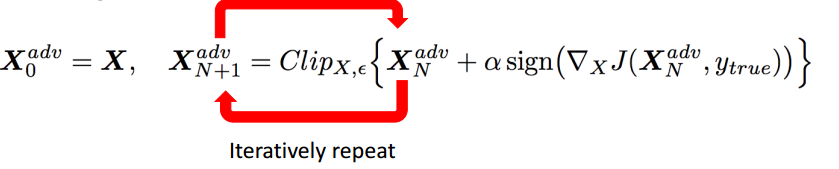
\includegraphics[scale=0.6]{iter_fgsm.png}
	\caption{Iterative FGSM Method \cite{goodfellow2016}.}
	\label{fig:iter_fgsm_craft}
\end{figure}
The extension of the fast method is reached by applying the gradient sign multiple times and clipping pixels that are not in the boundaries of the original image. Figure ~\ref{fig:iter_single_comp} shows the nature of perturbations of both methods. Since FGSM applies a single batch of perturbation to the image, it needs a higher amount of noise at a time to be able to successfully generate an adversarial.
\begin{figure}[!h]
	\centering
	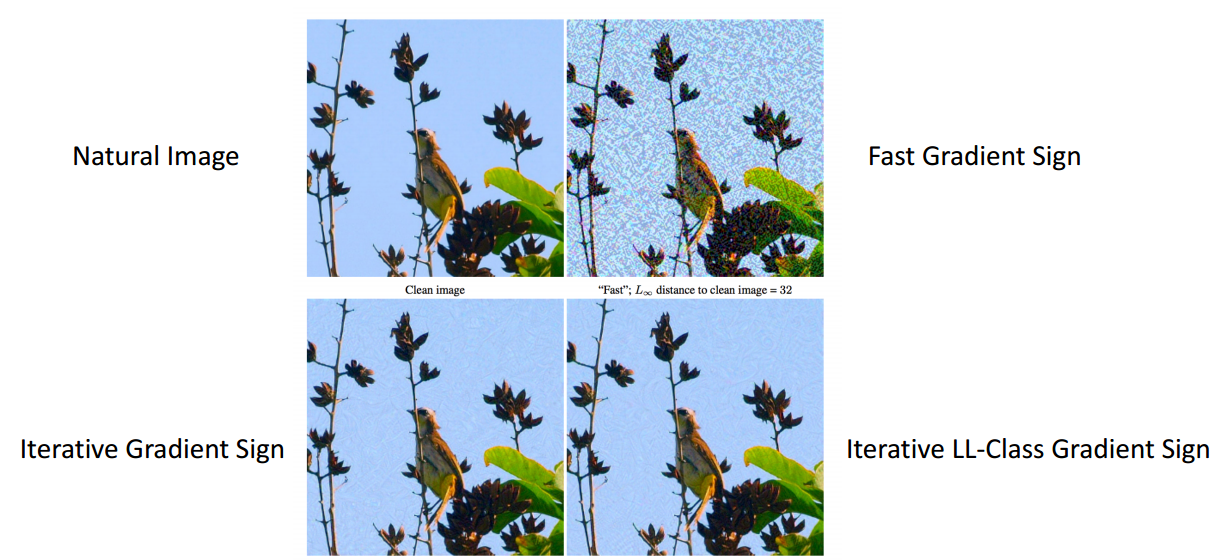
\includegraphics[scale=0.4]{iter_single.png}
	\caption{Visual Comparison of Gradients-based Methods \cite{goodfellow2016}.}
	\label{fig:iter_single_comp}
\end{figure}


\section{Ascent and descent perturbations}\label{sec:gsm}

Adding or subtracting intentional noise on images generates different adversaries,hence, requires different interpretations. By adding noise to an image, one would be making the gradient to go "uphill" and therefore moving away from the desired class, this results in an increase in value of the loss function and thus should be referred as the \textit{ascent method}. On the other hand, when subtracting intentional noise, one would be doing a process similar to the optimization of a loss function where we approach the minimum of a function and, thus, we get closer to the desired class, this approach is hereby known as the \textit{descent method}. These approaches can be coupled with iterative methods or fast methods to take progressive/single steps towards or away class labels. Some images/classes can be more robust to these perturbations and would, therefore, require more iterations or more noise from the gradient methods. Equations ~\ref{eq:ascent} and ~\ref{eq:descent} shows both ascent and descent methods 

\begin{equation}\label{eq:ascent}
C(x + \delta)\approx C(x) + \epsilon * sign(\nabla C)
\end{equation}
\begin{equation}\label{eq:descent}
C(x + \delta)\approx C(x) - \epsilon * sign(\nabla C)
\end{equation}